%%% Document class %%%
\documentclass[a4paper,12pt]{memoir}

%%% Packages %%%
\usepackage[margin=1.2in]{geometry}
\usepackage[utf8]{inputenc}
\usepackage[T1]{fontenc}
\usepackage[french]{babel}
\usepackage{enumitem}
\usepackage{hyperref}
\usepackage{listings}
\usepackage{graphicx}
\usepackage{xcolor}
\usepackage{tikz}
\usepackage{float}
\usepackage[Algorithme]{algorithm}
\usepackage{algpseudocode}
\usepackage{amsmath}
\usepackage{caption}
\usepackage{makeidx}
\usepackage{lmodern}
\usepackage{palatino}
\usepackage{amsfonts}
\usepackage{minted}
\usepackage{breakurl}
\usepackage{appendix}

\renewcommand\cftappendixname{\appendixname~}

%%% Configure minted package %%%

\definecolor{lbcolor}{rgb}{0.9,0.9,0.9}
\setminted{fontsize=\scriptsize,baselinestretch=1,breaklines,bgcolor=lbcolor}

%%% Translate algorithmic package %%%
\renewcommand{\algorithmicend}{\textbf{Fin}}
\renewcommand{\algorithmicif}{\textbf{Si}}
\renewcommand{\algorithmicthen}{\textbf{Alors}}
\renewcommand{\algorithmicelse}{\textbf{Sinon}}
\renewcommand{\algorithmicfunction}{\textbf{Fonction}}

%%% Define some commands %%%
\newcommand{\authors}[1]{\def\theauthors{#1}\author{#1}}
\newcommand{\supervisor}[1]{\def\thesupervisor{#1}}

\newcommand{\supervisorname}{Supervisor}
\addto{\captionsfrench}{\renewcommand{\supervisorname}{Superviseur}}


%%% Authors %%%
\authors{Simon Duret \texttt{<simon.duret@etu.u-bordeaux.fr>}\\
  Amélie Risi \texttt{<amélie.risi@etu.u-bordeaux.fr>} \\
  Brendan Guevel \texttt{<brendan.guevel@etu.u-bordeaux.fr}}

\supervisor{Aurélien Esnard \texttt{<aurelien.esnard@labri.fr>}}

%%%%% Report Title %%%%%
\title{Attaques sur connexions HTTPS}

%%% Header %%%
\newcommand{\authorname}{Auteurs}
\newcommand{\thepartname}{Partie}

\pretitle{\flushleft\Huge\textsf}
\posttitle{\\[-.65em]\rule{\linewidth}{1.5mm}\\[-.65em]
\centering
\vfill

\includegraphics{../medias/universite-bordeaux.pdf}
\vfill
{\Huge TER première année} \\
\vspace{1.25em}
\LARGE
Master \emph{Sciences et Technologies},\\
Mention \emph{Informatique},\\
Parcours \emph{Cryptologie et Sécurité Informatique}.\\
\par\hfill%
}

\preauthor{\vspace{\fill}\\
\flushleft\textbf{\large\authorname}\\
\small}
\postauthor{\vspace{1em}
  \newline\textbf{\large\supervisorname}\\\thesupervisor
\\[-.25em]
\rule{\linewidth}{1mm}\\[-.25em]}
\predate{\hspace{\fill}}
\postdate{}

%%% Chapters style %%%
\chapterstyle{veelo}


%%% Parts style %%%
\renewcommand*{\thepart}{\arabic{part}}
\renewcommand*{\parttitlefont}{\chaptitlefont\Huge}
\renewcommand*{\partnamefont}{\chapnamefont\HUGE}
\renewcommand*{\partnumfont}{\chapnumfont\HUGE}
\renewcommand{\beforepartskip}{\vspace*{\fill}}
\renewcommand{\midpartskip}{\vspace{.5em}\hrule height 1.5mm \vspace{.5em}}
\renewcommand{\afterpartskip}{\vspace*{\fill}}

%%% Table of contents style %%%
\renewcommand*{\cftpartname}{\thepartname}
\renewcommand*{\cftpartpresnum}{\space}
\renewcommand*{\cftpartaftersnum}{.}
\renewcommand*{\cftpartaftersnumb}{\space}

\cftpagenumbersoff{part}
\renewcommand{\cftpartafterpnum}{\protect\\[-.75em]%
  \protect\mbox{}\protect\hrule\par}

\renewcommand{\cftchapterdotsep}{4}

%%%%% Useful macros %%%%%
\newcommand{\latinloc}[1]{\ifx\undefined\lncs\relax\emph{#1}\else\textrm{#1}\fi\xspace}
\newcommand{\etc}{\latinloc{etc}}
\newcommand{\eg}{\latinloc{e.g.}}
\newcommand{\ie}{\latinloc{i.e.}}
\newcommand{\st}{\ensuremath{\text{\xspace s.t.\xspace}}}


%%% Hyperefs style %%%
\hypersetup{backref,
  pdfpagemode=FullScreen,
  colorlinks=true}

%%% Add some keywords to C language %%%
\lstdefinelanguage{Cext}{
  language     = C,
  morekeywords = {NULL, size_t},
}

%%% Code syntax highlighting (default) %%%
\lstset{
  frameround=fttt,
  language=Cext,
  numbers=left,
  breaklines=true,
  keywordstyle=\color{red}\bfseries,
  basicstyle=\ttfamily\color{blue},
  numberstyle=\color{black},
}

%%% Code syntax highlighting (shell) %%%
\lstdefinestyle{ShellStyle}{
  language=bash,
  basicstyle=\small\sffamily,
  numbers=none,
  numberstyle=\color{black},
  keywordstyle=\color{red}\bfseries,
  backgroundcolor=\color{yellow!18},
  linewidth=0.9\linewidth,
  xleftmargin=0.1\linewidth
}

%%% Code syntax highlighting (shell output) %%%
\lstdefinestyle{ShellOutputStyle}{
  language=sh,
  showspaces=false,
  showstringspaces=false,
  basicstyle=\small\sffamily,
  numbers=none,
  keywordstyle=\small\sffamily,
  backgroundcolor=\color{yellow!18},
  linewidth=0.9\linewidth,
  xleftmargin=0.1\linewidth
}

%%% Code syntax highlighting (python) %%%
\lstdefinestyle{PythonStyle}{
  language=python,
  basicstyle=\small\sffamily,
  numbers=none,
  numberstyle=\color{black},
  keywordstyle=\color{red}\bfseries,
  backgroundcolor=\color{yellow!18},
  linewidth=0.9\linewidth,
  xleftmargin=0.1\linewidth
}

%%% Document %%%
\begin{document}

\maketitle

\newpage

\tableofcontents*

\newpage

\chapter*{Introduction}
\addcontentsline{toc}{chapter}{Introduction}

Ce projet de TER a eu pour objectifs de s'intéresser aux attaques HTTPS, un protocole majoritairement utilisé de nos jours, développé en 1994 par Netscape. HTTPS est l'acronyme pour Hypertext Transfer Protocol over SSL. Il utilise le protocole HTTP, protocole de transfert hypertexte, ainsi qu'une couche de sécurisation. Cette couche est utilisée pour la confidentialité, l'intégrité et l'authentification du flux de données grâce aux protocoles SSL et TLS.

Le HTTPS permet à un visiteur de vérifier l'authenticité du site web qu'il visite grâce à un certificat d'authentification émis par une autorité tierce, réputée et de confiance. Théoriquement, il garantit la confidentialité et l'intégrité des données envoyées par l'utilisateur et reçues par le serveur. Dans un premier temps, les sites internet ont appliqué ce protocole seulement à des parties de leurs sites, par exemple pour le POST d'un formulaire. De nos jours, la majorité des sites proposant un accès restreint utilisent le HTTPS sur tout le site.

SSL et TLS sont deux protocoles cryptographiques utilisés dans la majorité des connexions sécurisées. Que ce soit pour l'accès à un serveur web via HTTPS, ou encore un envoi vers un serveur mail avec STARTTLS. SSL n'est cependant plus utilisé de nos jours, principalement à cause de l'attaque \hyperref[sec:poodle]{POODLE} qui a montrée des vulnérabilités critiques dans son implémentation en 2014. Depuis, le protocole TLS remplace ce dernier.

TLS utilise un schéma standard pour sécuriser une connexion :

\begin{itemize}
    \item Le client envoie une requête au serveur stipulant qu'il veut se connecter avec TLS.
    \item Un premier échange est fait pour décider de certains paramètres à utiliser pour la communication (chiffrement, fonction de hachage...).
    \item Le serveur fournit un certificat au client pour lui prouver son identité.
    \item Une fois l'identité confirmée par le client, les deux parties peuvent maintenant générer un secret commun, par exemple avec le chiffrement Diffie-Hellman. Ce secret partagé formera la clef de session.
    \item Grâce à cette clef de session, le client et le serveur peuvent maintenant communiquer de manière chiffrée et authentifiée en utilisant un chiffrement symétrique.
\end{itemize}

Malgré l'apparente sécurité du protocole TLS, il existe une multitude de points d'entrées qu'un attaquant peut utiliser pour récupérer une clef de session, ou usurper une connexion. Le but n'est généralement pas de chercher à casser RSA ou un autre chiffrement cryptographique. On va plutôt s'attaquer à certains détails de la communication, et failles dans la manière dont est gérée ces protocoles en pratique par les clients et les serveurs. Par exemple, l'attaque \hyperref[sec:poodle]{POODLE} utilise une faille dans la gestion de ces protocoles pour forcer les serveurs à sécuriser la connexion via SSL, au lieu de TLS, affaiblissant grandement la communication.

Au lieu de chercher à casser le chiffrement en son coeur, on va ainsi gratter tous les détails autour de l'implémentation qui peuvent permettre à un attaquant d'arriver à ses fins.

Dans ce rapport, nous proposons d'abord en première partie un état de l'art sur les principales attaques sur SSL et TLS, vues au cours des 15 dernières années. Puis nous aborderons l'essentiel de notre travail : une implémentation de plusieurs de ces attaques au travers de preuves de concepts (PoC). Ces PoC sont épurées dans le sens où les détails de l'attaque sont laissés de côté pour montrer le fonctionnement brut. Elles sont présentées sur des machines virtuelles, et sont accessibles pour n'importe qui voudrait les tester via un dépôt sur la plate-forme github : \url{https://github.com/t00sh/mastercsi-ter/}.

Nous aborderons donc trois versions de l'attaque SSLStrip, celle présentée en 2009 par Moxie Marlinspike, une extension pensée par LeonardoNve en 2014, et une dernière proposée par Jose Selvi en 2014. Puis, nous nous intéresserons à l'attaque HTTPS Interception.


\chapter{État de l'art des attaques sur SSL/TLS}

\begin{figure}[H]
  \caption{Historique des attaques SSL/TLS (source : Cloudflare \cite{cloudflare})}
  \fbox{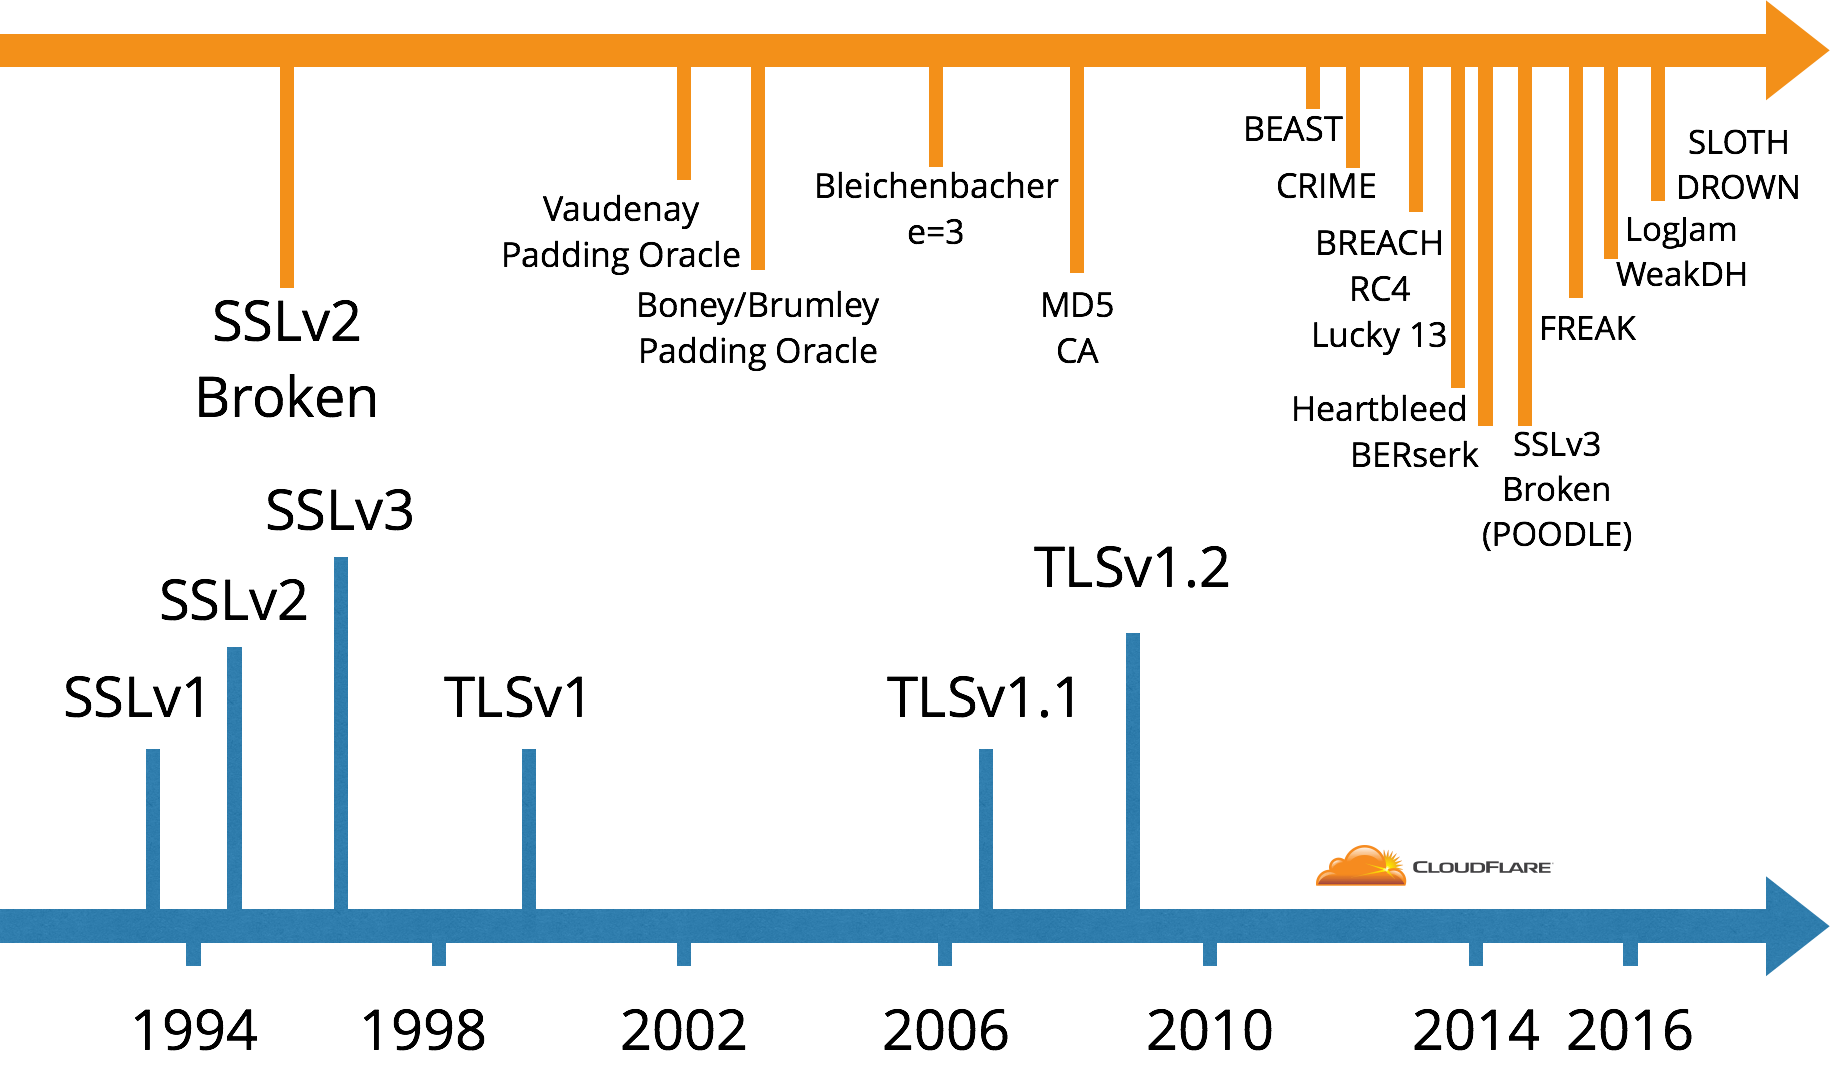
\includegraphics[width=\textwidth]{./history-tls-attacks.png}}
\end{figure}

\section{Attaques liées à l'implémentation}

\subsection{Heartbleed (2014)}

CVE-2014-0160

Il s'agit d'une vulnérabilité présente la bibliothèque cryptographique OpenSSL, notamment dans l'extension Heartbeat de SSL/TLS (RFC 6520). Ce protocole permet de maintenir la connection active (à la manière d'un ping), et une erreur de programmation dans la bibliothèque permettait de fuiter la mémoire d'un serveur. Ici, le client peut envoyer un paquet Heartbeat avec un champ ``longueur'' excédant la longueur réelle du paquet. Dans ce cas, le serveur vulnérable répondra avec un paquet contenant une partie de sa mémoire.

On pouvait donc récupérer à travers cette vulnérabilité un certains nombre d'informations confidentielles : clefs de sessions, clefs privées, cookies de sessions, mots de passe utilisateurs...\cite{heartbleed}.

\subsection{BERserk (2014)}

Cette faille concerne la bibliothèque Network Security Services présente dans certains navigateurs. L'attaque repose sur la falsification de signature numérique. La faille est présente à cause de l'analyse incorrecte de messages codés en ASN.1 lors de la vérification de signatures RSA.

Les messages ASN.1 sont constitués de diverses parties codées à l'aide de BER (Basic Encoding Rule) et DER (Distinguished Encoding Rules). C'est une variation de la faille Bleichenbacher PKCS\#1. Cette attaque exploite le fait que la longueur d'un champ dans le codage BER peut être utilisée pour utiliser de nombreux octets de données. Dans les implémentations vulnérables, ces octets sont ensuite ignorés lors de l'analyse.

Un attaquant peut donc se créer sa clé et se placer dans une situation de Man-In-TheMiddle. Dans ce cas, il intercepte les communications qui seront en clair pour lui car il aura chiffré celle-ci avec sa clé. Pour l'utilisateur, la connexion reste sécurisée et en plus, il verra toujours du https \cite{berserk}.

\section{Attaques liées à la cryptographie}

\subsection{BEAST (2011)}
L'attaque BEAST, Browser Exploit Against SSL/TLS concerne SSL 3.0 et TLS 1.0. L'attaquant, placé en Man-in-the-Middle, peut déchiffrer les données échangées entre le serveur et le client grâce à une vulnérabilité d'implémentation du mode CBC, Cipher Block Chaining. L'attaque se fait côté client en injectant des paquets dans le flux TLS. Cette technique est qualifiée d'attaque à clair connu. La faille du protocole réside dans le chiffrement par bloc. En effet, les blocs sont chiffrés les uns après les autres en utilisant le précédent \cite{beast}.

Voici le déroulement de l'attaque :

\begin{enumerate}
\item Injection du code chez la victime
\item La victime envoie de données forgées via SSL
\item L'attaquant écoute le trafic
\item Il renvoie les informations nécessaires à son code injecté
\item La victime renvoie les données forgées et on répète les deux étapes précédentes
  \item L'attaquant dérive tous les cookies
\end{enumerate}

\subsection{Cassage de RC4 (2013)}
RC4 est un algorithme qui était majoritairement utilisé pour protéger le traffic TLS.

La première attaque mise en place pour casser l'algorithme RC4 se base sur une multi-session attaque. C'est-à-dire que l'on a besoin d'envoyer un message clair cible à plusieurs reprise dans la même position dans le flux de texte lors de plusieurs connexions TLS. On exploite un octet sur le 256 initiaux des flux de clés RC4. Puisque les 36 premiers octets du texte clair sont formés à partir d'un message fini imprévisible, lorsque SHA-1 est l'algorithme de hachage séléctionné dans le protocle TLS, ces 36 premiers octets ne peuvent pas être récupérés. Cela signifie que l'attaque permet de récupérer 220 octets de textes clair cryptés par TLS. Le nombre de connexion nécessaires pour l'attaque peut être variable. L'attaquant peut mettre fin à la session TLS et certaines applications s'exécutant sur TLS puis se reconnecter automatiquement et retransmettre un cookie ou un mot de passe. Dans un environnement web, les sessions peuvent aussi être générées par des logiciels malveillants côté client, comme pour l'attaque BEAST.

La deuxième attaque s'applique à TLS et peut être effectuée grâce à une seule connexion. On exploite certains double octets dans le flux de clés RC4. On cible les octets en clair situés à n'importe quellle position dans le flux de texte clair TLS. Le nombre de cryptage nécessaire pour récupérer de façon fiable un ensemble de 16 octets de textes clair ciblés consécutifs est d'environ $10*2^{30}$, mais avec seulement $6*2^{30}$, ces octets peuvent être récupérer avec une fiabilité de 50\%. Cette attaque peut être plus efficace en pratique.

Dans cette attaque, l'attaquant peut se trouver dans n'importe où sur le chemin réseau entre le client et le serveur\cite{rc4}.

\subsection{Lucky13 (2013)}

Lucky 13 fait encore partie du cadre d'attaque MITM. La faille permet à un attaquant de récupérer du texte clair à partir d'une connexion TLS lorsque que le cryptage en mode CBC est utilisé. Comme l'attaque précédente, on effectue des attaques à plusieurs sessions, donc on a besoin d'envoyer un message clair cible à plusieurs reprise dans la même position dans le flux de texte lors de plusieurs connexions TLS. On détecte de petites différences dans l'heure à laquelle les messages d'erreur TLS apparaissent sur le réseau en réponse à des textes chiffrés générés par l'attaquant. L'attaquant doit récupérer plusieur échantillons pour une même heure car il y a souvent des perturbations.

Le nombre de session nécessaire est donc :

\begin{itemize}
\item 223 si l'attaquant se trouve sur le même LAN que la machine attaquée et que HMAC-SHA1 est utilisé comme algorithme MAC(Message authentication code) de TLS.
\item 219 si le texte clair est codé en base64.
\item 213 si un octet du texte clair dans l'une des deux dernières positions d'un bloc est déjà connu.
\end{itemize}
\cite{lucky13}.

\subsection{Logjam (2015)}

Logjam concerne l'algorithme Diffie-Hellman qui est mis en place lors du protocole TLS au moment du handshake. Cet algorithme permet d'échanger les clés et négocier la connexion sécurisée. L'attaquant, placé en MITM, peut écouter toutes connexions TLS qui utilisent de la crytographie basée sur 512 bits. L'attaque affecte les serveurs qui prennent en charge les chiffrements DHE\_EXPORT. Ce chiffrement requièrt un nombre premier court de 512 bits. Précisons que cette faiblesse a été créée volontairement pour satisfaire une réglémentation de années 90
\cite{logjam}.

\subsection{DROWN (2016)}

Drown(Decrypting RSA with Obsolete and Weakened eNcryption) affecte HTTPS, SSL et TLS. Lors de la découverte de cette attaque, les serveurs utilisait majoritairement TLS, néanmoins, ils supportaient aussi SSLv2. Cette prise en charge a constitué une menace, car l'attaquant peut déchiffrer des connexions TLS en envoyant des sondes à un serveur qui prend en charge SSLv2 et utilise la même clé. L'exploitation de cette faille passe par une attaque à chiffré choisi\cite{drown}.

\subsection{SLOTH (2016)}

Sloth(Security Losses from Obsolete and Truncated Transcript Hashes) s'intéresse à la perte de sécurité due à l'utilisation d'algorithmes de hachages obsolètes au sein des protocoles cryptographiques. Les algorithmes particulièrement ciblés sont SHA-1 et MD5 utilisés à cette époque dans TLS 1.1, TLS 1.2 et TLS 1.3 . Sloth est basée sur une attaque par collision par transposition et permet de réduire la sécurité de 128 bits à 64 bits\cite{sloth}.

\subsection{SWEET32 (2016)}

Sweet32 est une attaque qui vise des algorithmes de chiffrements utilisant des blocs de chiffrement inférieurs à 64 bits. Il faut utiliser encore une fois une attaque par collision. L'attaquant doit collecter aux maximum 32GB de données chiffrées qu'il doit analyser. Il peut donc trouver la clé privée et déchiffrer les message\cite{sweet32}.

\subsection{ROBOT (2017)}

Blablabla \cite{robot}

\section{Attaques sur le protocole}

\subsection{CRIME (2012)}

CRIME (compression ratio info-leak made easy), utilise une faille de l'algorithme de compression utilisé par TLS. Cette attaque vise surtout les cookies de sessions. L'idée est d'envoyer des caractères aléatoires dans un cookie forgé et de comparer la compression de ce dernier avec le cookie originel du client. Si le cookie forgé est partiellement compressé, on peut inférer qu'une partie de ce dernier correspondant au cookie du client. On procède ainsi par étapes successives pour retrouver le cookie et voler la session de la victime.

Cette attaque nécessite que l'attaquant se place en MITM pour pouvoir observer la taille du chiffré envoyé par le client mais également pouvoir envoyer des requêtes forgées par l'attaquant lui-même \cite{crime}.

\subsection{BREACH (2012)}

L'attaque BREACH (browser reconnaissance and exfiltration via adaptive compression of hypertext) est en grande partie similaire à CRIME vue plus haut. Cette fois ci ce n'est pas la compression TLS mais plutôt celle effectuée par HTTP qui est visée \cite{breach}.

\subsection{POODLE (2014)}

L'anagramme POODLE signifie "padding oracle on downgraded legacy encryption". L'attaque concerne surtout les chiffrements SSL 3.0, bien qu'une variante de la faille fut trouver sur TLS un pThe researchers’ paper describes a number of attacks that require some processing muscle, leaving them in the arena of well-resourced nation-state attackers for now. One transcript collision attack against TLS server signatures using MD5 cut the effective security in half from 128 bits to 64 bits. The security loss for other attacks against TLS authentication were worse, the researchers said, making such attacks much more practical.

“In all cases, the complexity of our transcript collision attacks are significantly lower than the estimated work for a second preimage attack on the underlying hash function. This definitively settles the debate on whether the security of mainstream cryptographic protocols depend on collision resistance,” the researchers wrote. “The answer is yes, cryptographers were right. Except in rare cases, mainstream protocols do require collision resistance for protection against man-in-the-middle transcript collision attacks. Consequently, we strongly recommend that weak hash functions like MD5 and SHA-1 should not just be deprecated; they should be forcefully disabled in existing protocols.”eu après.
Le padding dont parle le nom de l'attaque vient des méthodes de chiffrements cryptographiques. Lorsqu'un message envoyé un trop court pour l'algorithme de chiffrement, on lui rajoute une partie arbitraire, le "padding" pour qu'on puisse appliquer l'algorithme dessus.

Bien que le TLS soit un protocole plus sûr que SSL et recommandé aujourd'hui, de nombreux serveurs continuent d'accepter le SSL 3.0 si une connexion par TLS venait à être impossible. L'attaque POODLE se sert de ce fait pour forcer la connexion à se faire en SSL.

La vulnérabilité en elle-même vient de la façon dont sont encodés les blocs de donnés avec SSL. L'attaquant a besoin de deux choses pour se faire :

\begin{enumerate}
    \item L'attaquant doit pouvoir changer une partie du message injecté par le client dans l'algorithme
    \item Il doit avoir un retour sur le texte chiffré par SSL.
\end{enumerate}

Ces deux conditions peuvent s'exécuter avec par exemple une attaque en homme du milieu. L'attaquant doit toutefois avoir un contrôle également sur le client pour modifier le padding, ce qui est une tâche supplémentaire à effectuer.

En modifiant le padding, l'attaque permet de récupérer un byte d'information du message initial en envoyant un maximum de 256 requêtes. Cela peut amener l'attaquant à envoyer énormément de requêtes pour obtenir le message dans son intégralité.

L'avantage de cette attaque est qu'elle ne nécessite pas de connaître la clef utilisée pour le chiffrement \cite{poodle}.

\subsection{FREAK (2015)}

FREAK (factorising RSA export keys) a pour origine l'exportation de la cryptographie des USA qui gardait pour eux les meilleurs systèmes et partageait les moins bons avec le reste du monde, afin que la NSA puisse les craquer avec leur puissance de calcul supérieur.

Vers 2010 avec la montée en puissance constante des ordinateurs, tout le monde est maintenant capable avec un "bon pc" de craquer ces clés plus faibles, les "export-keys".

Le but de l'attaque est donc de forcer la connexion client/serveur de la victime a utiliser ces clefs plus faibles au lieu des clefs RSA standards plus fortes utilisées aujourd'hui \cite{freak}.

\subsection{WeakDH (2015)}

Blablabla \cite{weakdh}

\section{Attaques de l'homme du milieu}

\subsection{SSLsniff (2002)}

Blablabla \cite{sslsniff-website}

\subsection{SSLstrip (2009)}

Blablabla \cite{sslstrip-website}

\subsection{HTTPS interception}

Blablabla \cite{https-interception}


\chapter{Attaque SSLstrip}

\label{sec:sslstrip}

\begin{figure}[H]
  \caption{Attaque SSLstrip (diagramme Dia)}
  \fbox{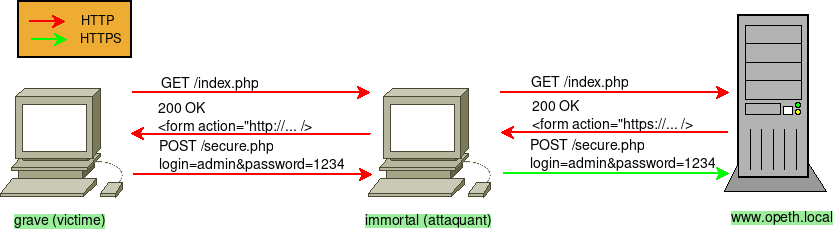
\includegraphics[width=\textwidth]{../medias/sslstrip/attack.png}}
\end{figure}

Le but de l'attaque est de rediriger tout trafic https vers du http sans que la victime s'en aperçoive. Il faut transformer tous les liens https en http et garder en mémoire tous les changement effectués.

Pour cela, il est nécessaire de se positionner en homme du milieu, avec par exemple une attaque de type ARP poisonning si l'on se trouve sur le même réseau local que la victime. L'attaque doit se passer soit lors des redirections 302, soit quand l'utilisateur clique sur un lien HTTPS.

Les actions à mettre en place sont les suivantes :

\begin{enumerate}
\item Regarder le trafic HTTP
\item Changer les liens https par des https et garder en mémoire les actions
\item Lorsque qu'on voit une requête HTTP pour une URL que l'on a supprimé, il faut envoyer au serveur du HTTPS
\item Conserver une carte des liens relatifs, CSS, JavaScript
\item Pour essayer de conserver le même aspect visuel, on doit faire de même pour les favicon en renvoyant la favicon de notre choix.
\item A éliminer des en-têtes de requêtes, les encodages, les cookies et les pages en cache.
\item Lors des requêtes POST envoyées par SSL, avec login et password, il faut faire expirer les cookies pour que l'utilisateur renvoie une requête sans cookies
\end{enumerate}

L'attaque SSLstrip a été présentée pour la première fois en 2009 par l'américain Moxie Marlinspike à la conférence en sécurité Blackhat. C'est une attaque très simple qui va permettre à un attaquant de pouvoir récupérer des informations confidentielles telles qu'un mot de passe ou un cookie de session. Cependant, l'attaque n'est plus vraiment d'actualité, nous reviendrons là dessus à la fin.

Pour que l'attaquant puisse utiliser sslstrip, il doit pouvoir se placer en homme du milieu entre le client et le serveur. C'est à dire qu'il doit être capable d'intercepter le trafic entre ces deux derniers, et pouvoir le modifier à sa guise. Bien sûr, l'attaquant n'a aucun intérêt à substituer une requête du client pour envoyer n'importe quoi à la place, car le serveur ne comprendra pas la requête et fermera la connexion TCP. Il va donc falloir être astucieux dans la manière dont on agit.

Pour pouvoir se placer en MITM, il y a plusieurs façons de procéder. Une des façons les plus simples consiste à se placer dans le réseau privé de la victime, et de faire de l'ARP spoofing/poisonning. L'idée étant de faire croire au routeur qu'il parle à la victime, et vice versa, en falsifiant leurs tables ARP respectives (cette table donnant la correspondance entre adresse mac et adresse ip). L'attaquant va ainsi pouvoir lire tout le trafic qui circule entre la victime et le routeur (donc entre la victime et le serveur).

Une fois placé en homme du milieu, l'attaquant peut donc voir et intercepter le trafic envoyé par la victime vers le serveur. Bien sûr, si ce trafic est chiffré, par exemple avec le protocol SSL/TLS, alors l'attaquant ne pourra rien en tirer, à moins de trouver une faille dans le chiffrement utilisé. Ici, on ne va pas essayer de casser TLS, mais plus de profiter du fait que toutes les requêtes envoyées par le client ne sont pas chiffrées (ce qui est de moins en moins le cas de nos jours).

Ainsi, si la requête du client est une simple requête http, l'attaquant va pouvoir lire ce qu'il envoie, et mieux encore, il va également voir la réponse du serveur.

On sait donc maintenant que notre attaquant peut, si la requête n'est pas chiffrée, lire l'échange effectué entre le client et le serveur, et même le modifier un peu si la requête reste valide et compréhensible par le serveur. Mais, qu'est-ce qu'on va bien pouvoir modifier pour obtenir des informations intéressantes ?

Pour répondre à cette question, il faut savoir que toutes les pages sensibles d'un site internet (qui demandent une connexion avec identifiant/mot de passe), ne sont accessibles généralement que par une requête sécurisée en https (ou alors le site est vraiment peu précautionneux). Lorsqu'une page html contient des liens vers des pages sécurisées, ces liens sont donc en https, pour indiquer au client qu'un chiffrement va être nécessaire à la connexion d'une page en particulier.

\begin{figure}[H]
  \caption{Exemple d'une page html avec un lien sécurité https}
  \fbox{\includegraphics[width=\textwidth]{../medias/sslstrip/screen2.png}}
\end{figure}

L'idée de l'attaque, va donc être de forcer le client à se connecter en http, et non en https, sur la page sensible. Pour cela, rien de plus simple : lorsque le serveur va envoyer une page html contenant des liens https, l'attaquant va simplement intercepter la page html, retirer le 's' de chacun de ces liens, et envoyer la page au client. Lorsque ce dernier voudra se connecter sur ces liens, il le fera donc en http et non en https comme il l'aurait fallu. L'attaquant va donc pouvoir lire tout le trafic de cette requête http, contenant par exemple un mot de passe si la page sécurisée était un formulaire de connexion.

\begin{figure}[H]
  \caption{La même page html, où l'attaquant a strip un 's'}
  \fbox{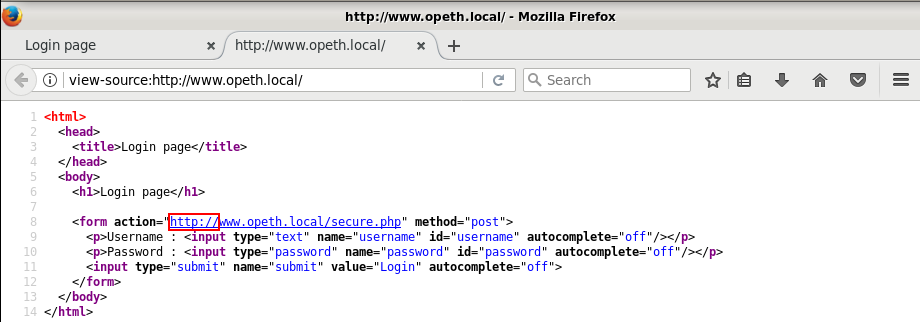
\includegraphics[width=\textwidth]{../medias/sslstrip/screen5.png}}
\end{figure}

*** recoper plus ou moins la description de l'attaque du README ? ***

Cependant, l'attaque n'est plus vraiment d'actualité car les sites internet modernes (ou plutôt, ceux qui pensent à la sécurité de leurs utilisateurs), utilisent https sur toutes les pages de leur site web, ce qui empêche l'attaquant d'intercepter ne serait-ce qu'une requête http, et de la modifier. De plus, une autre protection, nommée HSTS, permet au serveur d'indiquer à un client de toujours se connecter en https sur certaines pages. Ainsi, si un attaquant parvient à intercepter une requête http, et à remplacer les liens https vers des liens http dans le code html, le navigateur du client emettra une exception, car il aura gardé en mémoire qu'il doit se connecter en https sur tel domaine spécifique. Néanmoins il existe des moyens de contourner cet ajout, nous en parlerons dans la prochaine attaque.


\chapter{Attaque SSLstrip 2}

\label{sec:sslstrip2}

\begin{figure}[H]
  \caption{Attaque SSLstrip 2 (diagramme Dia)}
  \fbox{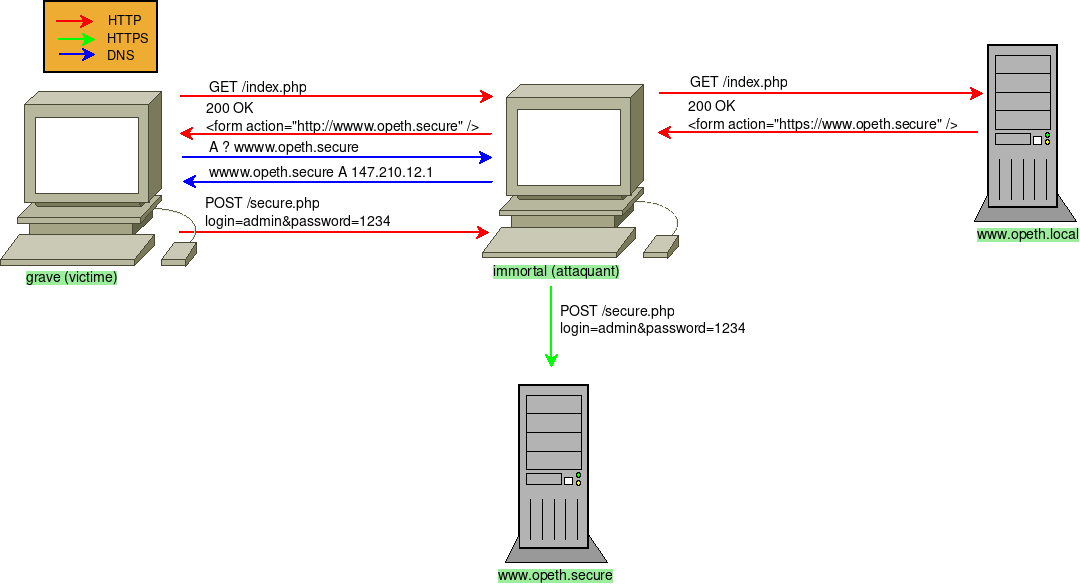
\includegraphics[width=\textwidth]{../medias/sslstrip2/attack.png}}
\end{figure}

Comme vu précédemment, une contre-mesure a été mise en place afin de déclarer aux clients d'un serveur qu'ils doivent utiliser une connexion sécurisée en HTTPS pour leur futures connexions avec celui-ci. Vous pouvez vous reporter à la section \hyperref[sec:hsts]{Contremesures} pour plus de précision.

Notre but est donc de contourner le HSTS en réutilisant l'attaque SSLStrip. Malheureusement, on ne peut pas la réutiliser directement car le navigateur a gardé en mémoire que toutes connexions sur cette page doivent se faire en HTTPS.

\section{Description de l'attaque}
Cette extension de SSLStrip a été pensée par LeonardoNve en 2014. Elle permet donc de passer au travers l'une des nouvelles contre-mesures mise en place sur les navigateurs. En effet, si l'attaquant se place en homme du milieu, il va pouvoir intercepter le trafic entre le client et le serveur afin de le faire réagir comme suit.

Lorsque le client va se connecter au serveur sur une page HTTP, l'attaquant va modifier cette page en remplaçant tous les liens HTTPS en HTTP mais aussi en changeant le nom de domaine. Changer le nom de domaine changera le comportement du navigateur. En effet, comme le navigateur ne connaît pas ce nom de domaine, il n'enverra pas d'exception liée à HSTS.

Voici un exemple :

Si le lien est \path{https://www.domain.secure}, on peut le remplacer par \path{http://wwww.domain.secure}.

Il faut noter que l'on enlève le \verb+s+ de \verb+https+ et que l'on remplace \verb+www+ par \verb+wwww+ ce qui change bien le nom de domaine.

Ainsi, l'attaquant fait croire au navigateur que cette requête est légitime et que \path{wwww.domain.secure} correspond au serveur distant. La connexion sera donc en HTTP et donc en clair.

\section{Notre attaque}

Tout d'abord, afin de pouvoir mettre en place l'attaque, il nous faut configurer l'environnement. Rappelons que l'attaquant est déjà positionné en homme du milieu, et que nous avons choisi de mettre sa machine dans le même réseau que la machine victime. Comme pour l'attaque précédente, nous utilisons l'outil \verb+qemunet+ développé par l'Inria qui nous permet de créer un environnement minimaliste et léger. Il nous faut donc vous expliquer sa mise en place.

\subsection{Mise en place de l'environnement}

\subsubsection{Configuration de la machine serveur - opeth}

Pour cette attaque, nous avons besoin d'un serveur DNS, installé sur la machine \textbf{opeth}. Pour cela, nous utilisons l'outil DNSMASQ. Le fichier \path{sslstrip2/opeth/dnsmasq.conf} spécifie notre nom de domaine et les actions relatives à la résolution du nom de domaine.

\inputminted[bgcolor=lbcolor, breaklines]{shell}{../sslstrip2/opeth/dnsmasq.conf}

On obtient donc le script de lancement suivant qui charge toutes les configurations et associe l'adresse IP de opeth aux noms de domaines suivants :

\begin{itemize}
\item \path{www.opeth.local} lorsque l'on accède en HTTP à la page ;
\item \path{www.opeth.secure} lorsque l'on accède en HTTPS.
\end{itemize}

\inputminted[bgcolor=lbcolor, breaklines]{shell}{../sslstrip2/opeth/start.sh}

\subsubsection{Configuration de la machine attaquante - immortal}


Cette machine utilise également DNSMASQ afin d'usurper les requêtes DNS de grave.

Comme précisé dans la description de l'attaque, nous avons besoin d'un nom de domaine supplémentaire afin de rediriger les requêtes DNS dessus. Ce nom de domaine est \path{wwww.opeth.secure}. On n'a donc besoin d'une règle dans la table PREROUTING de iptables afin de rediriger les paquets sur son propre serveur lorsque l'attaque à lieu.

Voici le contenu du fichier \path{/mnt/host/attack.sh} pour cette attaque :

\inputminted[bgcolor=lbcolor, breaklines]{shell}{../sslstrip2/immortal/attack.sh}

Nous commençons par rediriger les requêtes HTTP (port 80) sur le port de notre proxy (port 4242), puis les requêtes DNS sont redirigées vers le serveur DNS de l'attaquant.

\subsection{Démonstration}

Après ces présentations de mise en place, nous pouvons vous montrer le fonctionnement de l'attaque via une démonstration. Pour lancer l'environnement de test, il faut utiliser la commande suivante (on aura récupéré préalablement le dépôt \textbf{qemunet}) :

\begin{minted}{bash}
  ./qemunet/qemunet.sh -x -S sslstrip2
\end{minted}

Maintenant, nous avons les trois machines de lancées.

\subsubsection{Étape 1 : Avant l'attaque}

Avant de vous montrer ce qu'il se passe lors de l'attaque, nous devons vous montrer l'état initial et le fonctionnement de HSTS.

Lorsque l'attaque n'est pas lancée, et que c'est la première fois que nous visitons le domaine \path{www.opeth.secure}, nous voyons que nous pouvons utiliser le protocole HTTP :

\begin{figure}[H]
  \caption{Visite du domaine en HTTP, lors de la première connexion}
  \fbox{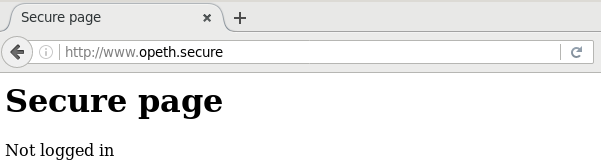
\includegraphics[width=\textwidth]{../medias/sslstrip2/screen1.png}}
\end{figure}

Par contre, une fois que le site a été visité en HTTPS une fois et grâce à HSTS, il est alors impossible d'accéder de nouveau au domaine \path{www.opeth.secure} en HTTP. Firefox effectuera automatiquement la requête en HTTPS :

\begin{figure}[H]
  \caption{Visite du domaine en HTTP, lorsqu'il a été sécurisé avec HSTS}
  \fbox{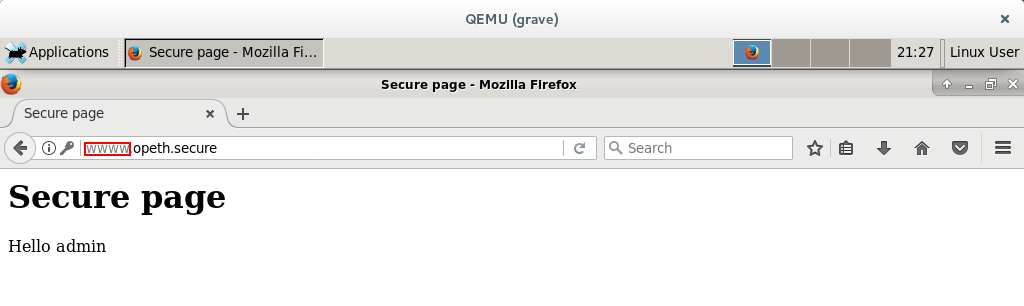
\includegraphics[width=\textwidth]{../medias/sslstrip2/screen2.png}}
\end{figure}

Nous voyons donc que même sur une URL en \path{http://www.opeth.secure}, si l'entrée HSTS existe nous serons tout de même connecté automatiquement en HTTPS.

\subsubsection{Étape 2 : lancement de l'attaque}

Comme expliqué précédemment, pour lancer l'attaque, il faut exécuter le fichier \path{/mnt/host/attack.sh} depuis immortal dont on a déjà expliqué son comportement.

Nous pouvons maintenant lancer l'attaque depuis la machine immortal :


\begin{figure}[H]
  \caption{Lancement de l'attaque}
  \fbox{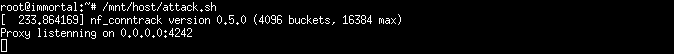
\includegraphics[width=\textwidth]{../medias/sslstrip2/screen4.png}}
\end{figure}

\paragraph{Explication du code \\}

Le code du proxy est dans le dossier de la machine immortal, le fichier \path{sslstrip2.py}.

\subparagraph{Réception des requêtes \\}

Lors de la réception de requêtes, il s'agit de savoir si l'on doit :

\begin{itemize}
\item fermer la connexion (le client ou le serveur a fermé la connexion)
\item établir une connexion en HTTPS, dans le cas où le client va sur le domaine \path{wwww.opeth.secure}
  \item établir une connexion HTTP, dans le cas où le client demande la page du domaine \path{www.opeth.local}
\end{itemize}

La fonction traitant les différentes requêtes est celle-ci :

\begin{minted}{python}
def __recv(self, csock):
        fw_sock = self.__csockets[csock]
        data = csock.recv(BUFFER_SIZE)
        if len(data) == 0:
            self.__close_conn(csock)
            self.__close_conn(fw_sock)
        else:
            print(data)

            if fw_sock is None:
                m = re.search(b'Host: (\S+)', data)
                if m is not None and m.group(1) == FAKE_HOST:
                    re.sub(b'Host: (\S+)',
                           b'Host: ' + bytes(FORWARD_HOST_HSTS), data)
                    self.__new_https_conn(csock)
                else:
                    self.__new_http_conn(csock)
                fw_sock = self.__csockets[csock]
            data = self.__replace_https_to_http(data)
            data = self.__replace_host(data)
            data = self.__replace_content_length(data)
            fw_sock.send(data)
\end{minted}

À la fin, on transforme tous les liens HTTPS trouvés en HTTP en remplaçant le nom de domaine \path{www.opeth.secure} par le faux nom de domaine \path{wwww.opeth.secure}, on met l'entête Host vers le bon domaine et on recalcule la taille de la requête (entête Content-Lenght)

\subparagraph{Transformation des liens \\}

Dans cette fonction, nous utilisons une expression régulière afin de remplacer tous les liens \path{https://www.opeth.secure} en \path{http://wwww.opeth.secure}.

\begin{minted}{python}
def __replace_https_to_http(self, data):
    return re.sub(b'https://' + bytes(FORWARD_HOST_HSTS),
                  b'http://' + bytes(FAKE_HOST), data)
\end{minted}

\subparagraph{Modification de l'entête Host}

Lorsque la victime est redirigée vers un lien \path{http://wwww.opeth.secure}, l'entête Host de ses requêtes sera erronée. Cette fonction modifie cette entête pour que le serveur puisse recevoir un Host correct.

\begin{minted}{python}
def __replace_host(self, data):
    return re.sub(b'Host: ' + bytes(FAKE_HOST),
                  b'Host: ' + bytes(FORWARD_HOST_HSTS), data)
\end{minted}


\subparagraph{Recalcul de l'entête Content-Length}

La taille de la requête étant modifiée par le proxy, celui-ci doit recalculer l'entête Content-Length en se basant sur la chaîne "{\textbackslash}r{\textbackslash}n{\textbackslash}r{\textbackslash}n" signalant la fin des entêtes dans le protocole HTTP.

\begin{minted}{python}
def __replace_content_length(self, data):
    try:
        idx = data.index(b"\r\n\r\n")
        length = len(data) - idx - 4
        return re.sub(b'Content-Length: (\d+)',
                      b'Content-Length: %d' % length, data, 1)
    except:
        return data
\end{minted}

\subsubsection{Étape 3 : Pendant l'attaque}

Lorsque l'attaque est lancée, on peut voir que le lien sensible \path{https://www.opeth.secure} est remplacé par \path{http://wwww.opeth.secure}.
La machine immortal est donc capable d'intercepter les échanges réalisés sur le domaine \path{www.opeth.secure}.

Dans cette image, on voit dans l'encadré rouge, que le lien \path{https://} a bien été remplacé par un lien non sécurisé \path{http://} :

\begin{figure}[H]
  \caption{Le 's' de "https" a disparu}
  \fbox{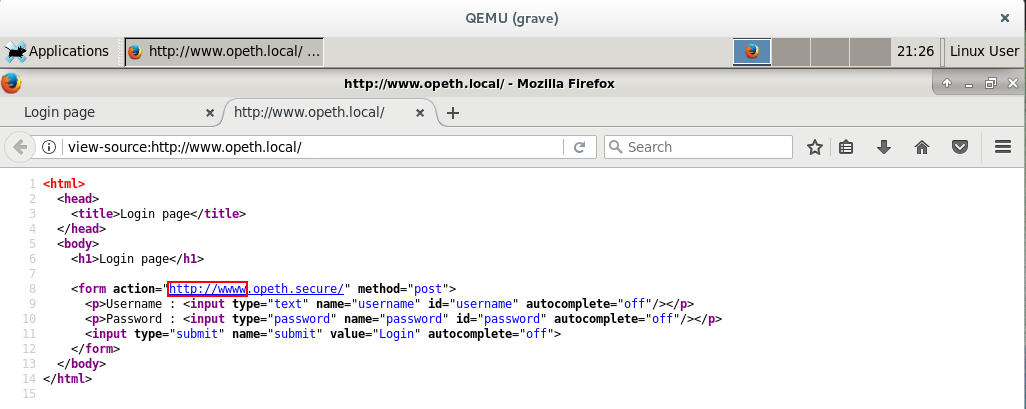
\includegraphics[width=\textwidth]{../medias/sslstrip2/screen5.png}}
\end{figure}

Nous constatons que nous arrivons sur la page secure.php en HTTP : notre navigation n'est pas sécurisée !

\begin{figure}[H]
  \caption{Le client visite une page sécurisée en http}
  \fbox{\includegraphics[width=\textwidth]{../medias/sslstrip2/screen6.png}}
\end{figure}

La machine immortal a été capable de capturer non seulement les identifiants du formulaire, mais également le cookie de session :

\begin{figure}[H]
  \caption{L'attaquant récupère toutes les informations sensibles}
  \fbox{\includegraphics[width=\textwidth]{../medias/sslstrip2/screen7.png}}
\end{figure}

Le script complet de l'attaque peut être consulté à l'annexe \ref{appendix:sslstrip2}.

\section{Limitations de notre attaque}

Dans cette attaque, nous ajoutons au domaine attaqué un 'w' en passant de \path{www.opeth.secure} à \path{wwww.opeth.secure}. Un utilisateur un petit peu averti, verra sans doute la supercherie. Suivant le domaine attaqué, un choix plus judicieux pourrait sans doute passer plus inaperçu.

Nous avons également fait la supposition que l'attaquant a la possibilité d'usurper les requêtes DNS du client. Suivant où est placé l'attaquant sur le réseau, ceci ne sera peut être pas possible et l'attaque ne pourra donc pas être réalisée.

Ce script possède également les même limitations que celui sur \hyperref[sec:sslstrip]{SSLStrip}.


\chapter{SSLStrip NTP}

\label{sec:sslstrip-ntp}

\begin{figure}[H]
  \caption{Attaque SSLStrip NTP (diagramme Dia)}
  \fbox{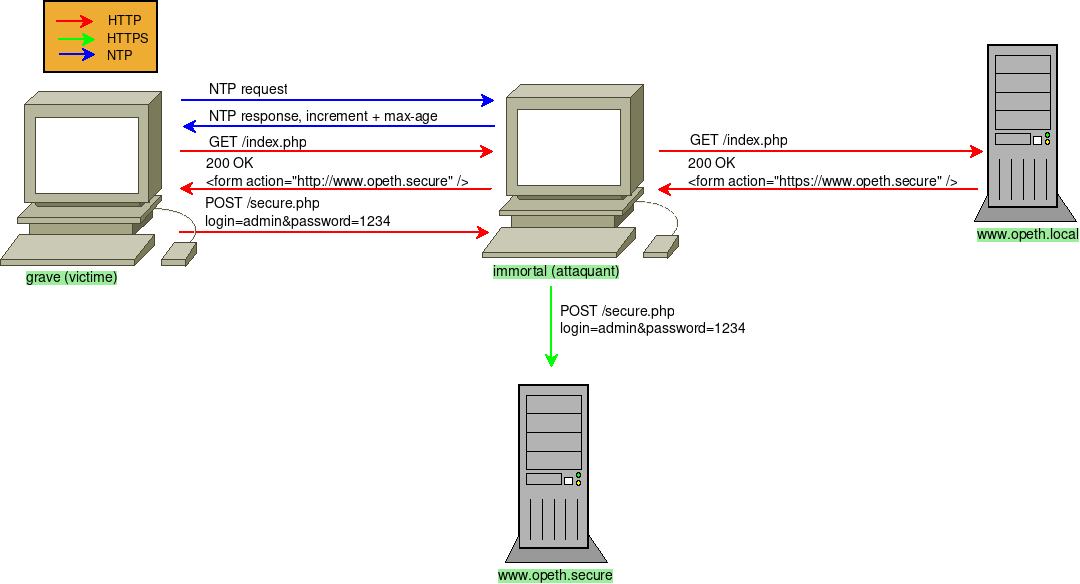
\includegraphics[width=\textwidth]{../medias/sslstrip-ntp/attack.png}}
\end{figure}

\section{Description de l'attaque}

Cette nouvelle amélioration de l'attaque SSLStrip a été présentée lors de la BlackHat Europe par Jose Selvi. Celle-ci utilise le protocole NTP afin de contourner la sécurité offerte par HSTS.

L'attaque SSLStrip originale n'est en effet plus possible lorsque l'on essaye de "stripper" les URL d'une page web d'un domaine qui a été protégé ultérieurement par HTTP Strict Transport Security. Le mécanisme HSTS va obliger le client à se connecter à l'URL que l'on cherche à stripper en HTTPS pendant un certain laps de temps (défini par le serveur), rendant l'attaque complètement inefficace.

Le protocole NTP (Network Time Protocol) permet de synchroniser l'horloge d'un équipement informatique avec un serveur NTP. Il s'agit d'un protocole sans états basé sur UDP et absolument pas sécurisé. L'attaque présentée par Jose Selvi consiste à usurper les requêtes NTP pour renvoyer une date erronée au client, et ainsi faire expirer les entrées HSTS. Pour réaliser cela, l'auteur se base sur un outil Python appelé Delorean, qui se comporte comme un serveur NTP et pour lequel on peut définir la date de réponse.

Une fois que l'horloge du client a été compromise et le HSTS du domaine expiré, il est possible d'utiliser l'attaque SSLStrip originale afin de stripper les URL des pages web, même pour les domaines censés être protégés par HSTS.

\section{Notre attaque}

Dans ce projet de TER, nous avons eu à réaliser une preuve de concept de cette attaque. Voici les détails de notre implémentation.

\subsection{Mise en place de l'environnement}

Pour résoudre les différents domaines, nous utilisons le fichier \path{/etc/hosts} de chaque machine.

\subsubsection{Configuration de la machine serveur - opeth}

Pour cette attaque, nous avons ajouté un serveur NTP légitime sur la machine \textbf{opeth}, à travers l'outil ntpd. La configuration de base était suffisante pour notre démonstration. À noter que dans la réalité, le serveur NTP aurait été probablement sur une machine différente.

Concernant le serveur web NGINX, celui-ci utilise les deux domaines \path{www.opeth.local} et \path{www.opeth.secure}. Le premier est accédé en HTTP alors que le second en HTTPS et protégé grâce à HSTS.

\subsubsection{Configuration de la machine cliente - grave}

Il a fallut utiliser un client NTP sur cette machine pour cette attaque. Nous utilisons donc sntpc (Simple NTP Client), que l'on lance au démarrage de la machine et que l'on configure pour effectuer ses requêtes vers \textbf{opeth} de manière régulière (toutes les secondes pour les besoins de la démonstration).


\subsubsection{Configuration de la machine attaquante - immortal}

C'est sur cette machine que se trouve la preuve de concept de l'attaque. Nous avons également utilisé le script Delorean \cite{delorean} comme décrit dans le papier de l'attaque afin d'usurper les requêtes NTP de la machine grave. L'attaque se lance grâce au script \path{/mnt/host/attack.sh} :

\inputminted[bgcolor=lbcolor, breaklines]{bash}{../sslstrip-ntp/immortal/attack.sh}

Nous commençons par rediriger les requêtes HTTP sur le port de notre proxy, puis les requêtes NTP vers le port de Delorean. Nous calculons ensuite le temps d'expiration des entrées HSTS à l'aide de l'outil curl. Finalement, nous lançons le serveur Delorean ainsi que notre proxy implémentant l'attaque SSLStrip.

\subsection{Démonstration}

Dans cette partie, nous allons illustrer l'attaque SSLStrip NTP dans l'environnement que nous avons mis en place. Pour lancer l'environnement de test, il suffit de lancer qemunet de la manière suivante :

\begin{minted}{bash}
./qemunet/qemunet.sh -x -S sslstrip-ntp
\end{minted}

À partir de là, les trois machines sont lancées.

\subsubsection{Étape 1 : avant l'attaque}

Lorsque l'attaque n'est pas encore lancée, nous pouvons voir sur la machine grave que tout se passe normalement et que la requête POST passe bien en HTTPS ; immortal est donc incapable de voir les identifiants envoyés :

\begin{figure}[H]
  \caption{Attaque SSLStrip NTP (avant l'attaque)}
  \fbox{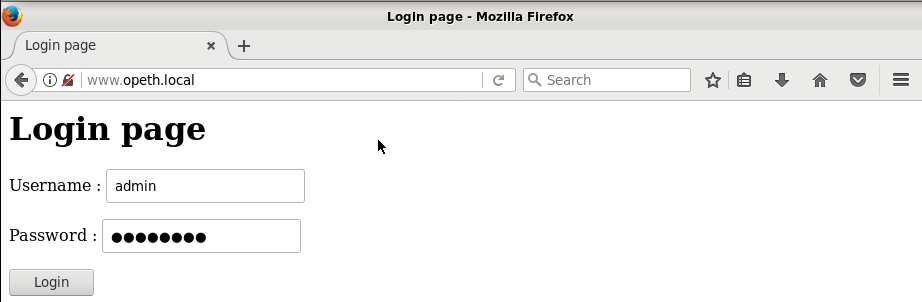
\includegraphics[width=\textwidth]{../medias/sslstrip-ntp/screen1.png}}
\end{figure}


L'encadré rouge ci-dessous montre bien que le POST est effectué en HTTPS, sur le domaine \path{www.opeth.secure}. Lorsque nous affichons le code source de la page, nous obtenons :

\begin{figure}[H]
  \caption{Code source de la page (avant l'attaque)}
  \fbox{\includegraphics[width=\textwidth]{../medias/sslstrip-ntp/screen2.png}}
\end{figure}

Nous arrivons alors sur le domaine \path{www.opeth.secure} en HTTPS : immortal n'a pas pût voir nos échanges sur cette page sécurisée comme le montre la figure ci-dessous.

\begin{figure}[H]
  \caption{La connexion se fait bien en HTTPS}
  \fbox{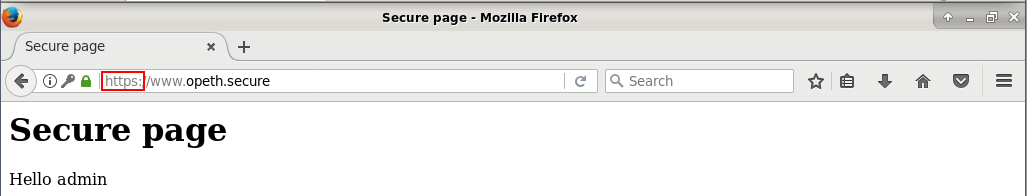
\includegraphics[width=\textwidth]{../medias/sslstrip-ntp/screen3.png}}
\end{figure}

\subsubsection{Étape 2 : pendant l'attaque}

Lorsque l'attaque est en cours et quand le client réalisera une requête NTP, celle-ci va être redirigée vers Delorean qui répondra avec une date permettant de faire expirer son entrée HSTS. Ensuite, quand la machine grave visitera la page non-sécurisée \path{www.opeth.local}, tous les liens HTTPS vers \path{www.opeth.secure} seront strippés.

Ici on voit dans le code source de la page que notre proxy a remplacé les liens \path{https://} par \path{http://}.

\begin{figure}[H]
  \caption{Code source de la page (pendant l'attaque)}
  \fbox{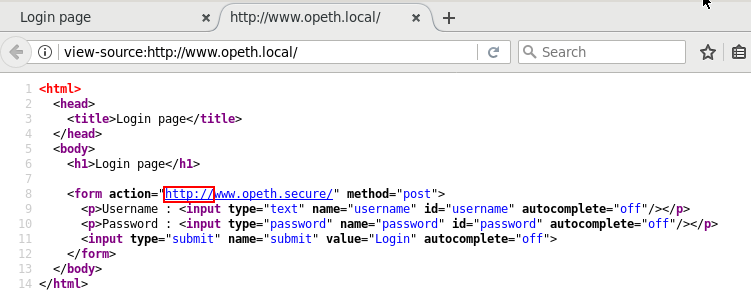
\includegraphics[width=\textwidth]{../medias/sslstrip-ntp/screen5.png}}
\end{figure}

Nous constatons que nous arrivons sur le domaine \path{www.opeth.secure} en HTTP : notre navigation n'est pas sécurisée !

\begin{figure}[H]
  \fbox{\includegraphics[width=\textwidth]{../medias/sslstrip-ntp/screen6.png}}
\end{figure}

La machine immortal a été capable de capturer non seulement les identifiants du formulaire, mais également le cookie de session alors que le domaine était protégé par HSTS :

\begin{figure}[H]
  \fbox{\includegraphics[width=\textwidth]{../medias/sslstrip-ntp/screen7.png}}
\end{figure}

Le script complet de l'attaque peut être consulté à l'annexe \ref{appendix:sslstrip-ntp}.

\section{Limitations de notre attaque}

Dans cette attaque, nous supposons que le client effectue des requêtes NTP. Ceci n'est en fait pas toujours le cas, et il arrive que des clients n'utilisent pas NTP pour mettre leur horloge à jour.

De plus, ici notre attaque fonctionne relativement rapidement car notre client a été configuré pour effectuer ses requêtes toutes les secondes. En pratique, l'attente d'une requête NTP peut être beaucoup plus longue et est souvent de l'ordre de plusieurs heures.

Une autre supposition que nous avons faite mais qui n'est peut être pas possible en réalité est que nous sommes sur le chemin entre le client et le serveur NTP. Suivant à quel endroit l'attaquant a réussi à se placer en homme du milieu, l'attaque pourrait ne pas être possible.

Ce script possède également les même limitations que celui sur \hyperref[sec:sslstrip](SSLStrip).


\chapter{Interception HTTPS}

\label{sec:https-interception}

\begin{figure}[H]
  \caption{Attaque HTTPS interception (diagramme Dia)}
  \fbox{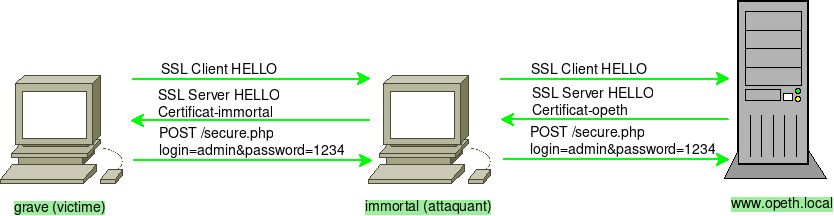
\includegraphics[width=\textwidth]{../medias/https-interception/attack.png}}
\end{figure}

\section{Description de l'attaque}

La méthode que nous allons voir pour intercepter un trafic HTTPS n'est pas vraiment une attaque. Pour être menée à bien, la machine, placée en homme du milieu, doit avoir installée sa propre autorité de certification, et surtout l'avoir rentrée sur la machine du client, en amont.

C'est une chose qui peut être assez dure à réaliser pour un attaquant, mais il existe des cas où cette situation peut se présenter. Dans le cadre d'une entreprise, il n'est pas rare que les requêtes HTTP des employés passent par un proxy, pour suivre leurs activités. Les responsables n'ont par contre, a priori pas moyen de lire les requêtes HTTPS, du moins c'est ce qu'on pourrait penser.

Car c'est en fait au contraire assez simple à réaliser dans la mesure où il est facile de rajouter une autorité de certification à la main dans les navigateurs web de tous les employés.

L'idée de la méthode est d'agir comme un simple proxy HTTPS. Lors de la connexion initiale du client vers le site web, la machine placée en homme du milieu va récupérer la requête, et établir elle même une connexion avec le serveur distant. Le proxy n'a plus qu'à établir une connexion avec le client, ce qui ne pose pas de problème car l'autorité de certification est acceptée par le navigateur du client.

Par ailleurs, l'ANSSI a publié une ressource à destination des entreprises sur comment intercepter le trafic HTTPS de ses employés \cite{anssi}.
\section{Notre attaque}

\subsection{Mise en place de l'environnement}

Le serveur \textbf{opeth} héberge deux pages sur le domaine \path{www.opeth.local} :

\begin{itemize}
\item une page \path{index.php} que l'on accède en HTTPS et présentant un formulaire de login ;
\item une page \path{secure.php} que l'on accède en HTTPS depuis la page \path{index.php}.
\end{itemize}

Pour la résolution DNS, nous utilisons simplement le fichier \path{/etc/hosts} de chaque machine. Nous avons également mis en place HSTS sur cette attaque, étant donné que nous traitons uniquement des flux HTTPS.

\subsection{Démonstration}

On peut lancer l'environnement de test grâce à cette commande :

\begin{minted}{bash}
./qemunet/qemunet.sh -x -S https-interception
\end{minted}

À partir de là, les trois machines sont lancées.

\subsubsection{Étape 1 : avant l'attaque}

Avant que l'attaque soit lancée, nous pouvons accéder à la page de login de manière sécurisée. La machine immortal n'est pas capable de comprendre la communication entre le client (grave) et le serveur (opeth) :

\begin{figure}[H]
  \caption{Attaque https-interception (avant l'attaque)}
  \fbox{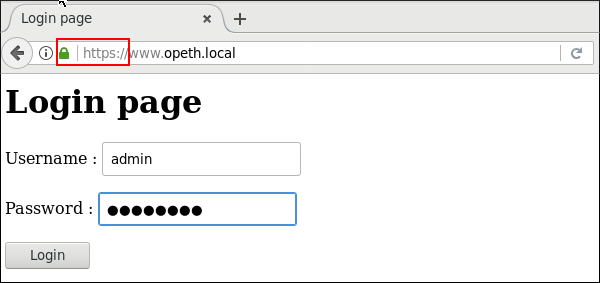
\includegraphics[width=\textwidth]{../medias/https-interception/screen1.png}}
\end{figure}

Ici, on voit que c'est bien le certificat du serveur qui est présenté au navigateur :

\begin{figure}[H]
  \caption{Certificat}
  \fbox{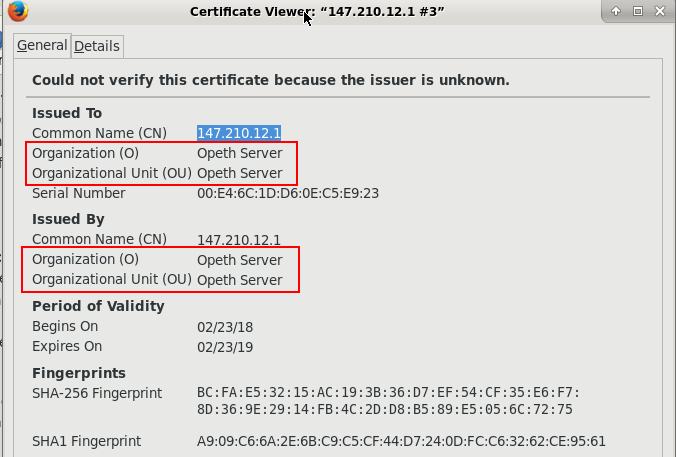
\includegraphics[width=\textwidth]{../medias/https-interception/screen2.png}}
\end{figure}

Nous voici sur la page \path{secure.php}, nos données ont transitées de manière chiffrées entre le client et le serveur :

\begin{figure}[H]
  \caption{HTTPS se présente normalement}
  \fbox{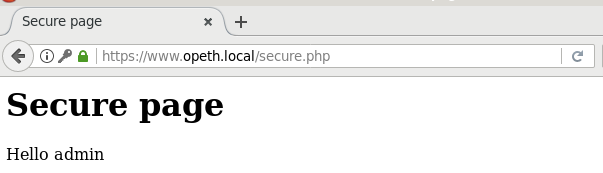
\includegraphics[width=\textwidth]{../medias/https-interception/screen3.png}}
\end{figure}


\subsubsection{Étape 2 : lancement de l'attaque}

Comme expliqué précédemment, pour lancer l'attaque, il faut exécuter le fichier \path{/mnt/host/attack.sh} depuis immortal. Voici son contenu :

\begin{minted}{bash}
PROXY_PORT=4242

iptables -t nat -F
iptables -t nat -A PREROUTING -d 147.210.12.1 -p tcp --dport 443 -j REDIRECT --to-port $PROXY_PORT
/mnt/host/https-interception.py $PROXY_PORT
\end{minted}

On peut constater que les flux TCP à destination du port 443 (HTTPS) sont redirigées vers le port d'écoute du proxy qui est chargé d'analyser et traiter les requêtes.

Sur la machine immortal, nous lançons le script de l'attaque :

\begin{figure}[H]
  \caption{Lancement de l'attaque}
  \fbox{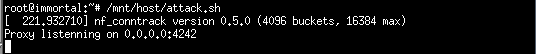
\includegraphics[width=\textwidth]{../medias/https-interception/screen4.png}}
\end{figure}

\paragraph{Explication du code du proxy \\}

Le code du proxy est dans le fichier \path{https-interception.py}. Ce dernier est sensiblement le même que celui utilisé pour l'attaque SSLStrip.

\subparagraph{Contexte SSL du proxy \\}

Le proxy doit ajouter son certificat au contexte pour pouvoir le présenter au client :

\begin{minted}{python}
def __listen(self):
	sock = socket.socket()
	context = ssl.create_default_context(ssl.Purpose.CLIENT_AUTH)
	context.load_cert_chain(certfile=PROXY_CERT, keyfile=PROXY_KEY)
	...
\end{minted}

\subsubsection{Étape 3 : pendant l'attaque}

Lorsque l'attaque est en cours, le certificat présenté au client n'est plus celui d'opeth, mais celui du proxy, signé par l'autorité de certification. À noter qu'ici si l'autorité de certification du proxy n'avait pas été présent dans le navigateur, celui-ci aurait émis une alerte.

Ci-dessous on voit que le certificat présenté est celui du proxy (immortal), et non plus celui du serveur. On voit bien que les empreintes SHA256 sont différentes.

\begin{figure}[H]
  \caption{Le certificat a changé}
  \fbox{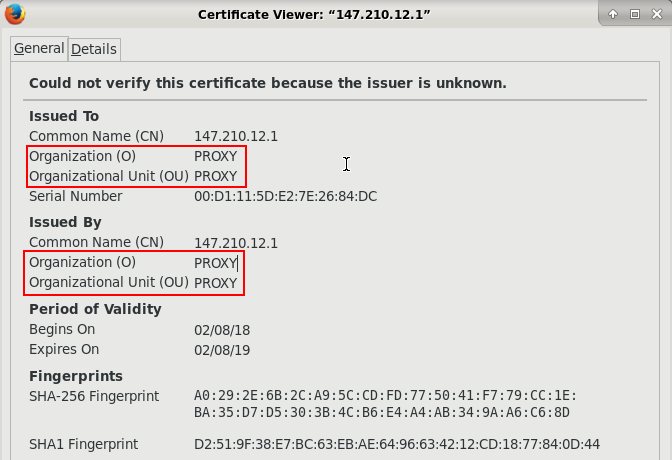
\includegraphics[width=\textwidth]{../medias/https-interception/screen6.png}}
\end{figure}

Si le certificat est accepté par le client et que nous essayons de nous enregistrer :

\begin{figure}[H]
  \caption{Connexion sécurisée}
  \fbox{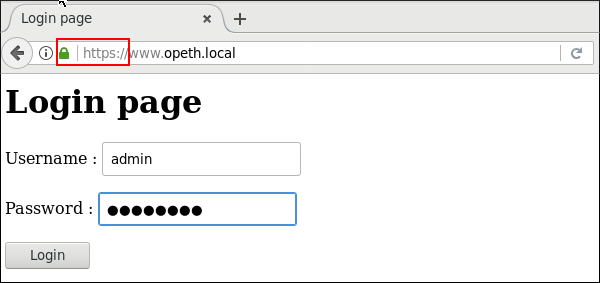
\includegraphics[width=\textwidth]{../medias/https-interception/screen1.png}}
\end{figure}

Nous arrivons bien sur la page \path{secure.php}, et notre connexion est bien effectuée en HTTPS. Le client n'a constaté aucun changement au niveau de sa navigation.

\begin{figure}[H]
  \caption{Tout a l'air normal pour le client}
  \fbox{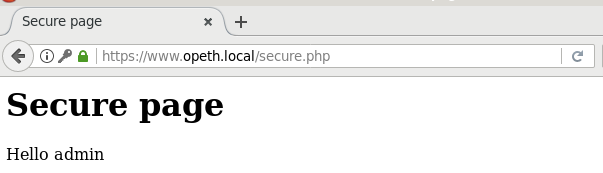
\includegraphics[width=\textwidth]{../medias/https-interception/screen3.png}}
\end{figure}

Par contre, la machine immortal a jouée le rôle d'un proxy et a été capable de récupérer la communication en clair. Ici on voit que le nom d'utilisateur, le mot de passe ainsi que le cookie de session ont pût être capturés :

\begin{figure}[H]
  \caption{L'attaquant a intercepté les informations sensibles}
  \fbox{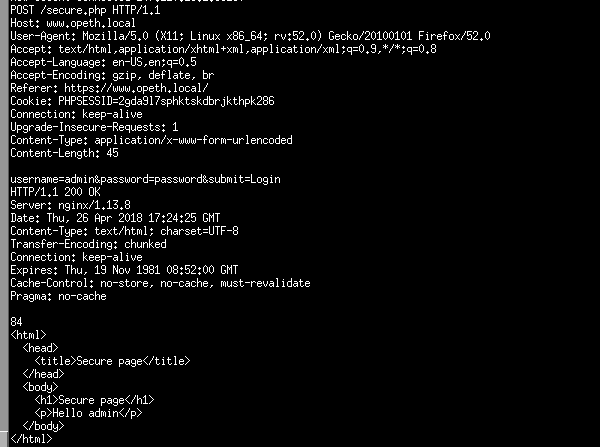
\includegraphics[width=\textwidth]{../medias/https-interception/screen9.png}}
\end{figure}

Le script complet de l'attaque peut être consulté à l'annexe \ref{appendix:https-interception}.

\section{Limitations de notre attaque}

Notre attaque étant une preuve de concept, celle-ci présente un certain nombre de limitations. Dans un premier temps, nous avons supposé qu'il était possible d'installer un certificat sur le navigateur du client. Ceci est bien entendu possible pour les administrateurs de postes clients d'une entreprise. Certains antivirus utilisent également cette technique afin d'analyser le trafic HTTPS d'une machine.

Mais dans la majorité des cas, ceci n'est pas une option. Pour contourner ce problème, soit l'attaquant proposera un certificat qui ne pourra pas être signé par une autorité de certification, et celui-ci déclenchera alors une alerte sur le navigateur du client concerné. Soit l'attaquant cherchera à pirater une autorité de certification publique, dans le but de générer des certificats frauduleux pour des domaines légitimes. Cette dernière possibilité est sans doutes la plus compliquée et la moins réaliste.


\chapter*{Conclusion}

\addcontentsline{toc}{chapter}{Conclusion}

Dans ce rapport de TER, nous présentons un état de l'art, ainsi que 4 preuves de concepts implémentant des attaques sur https. Ces dernières ne fonctionnent que dans des conditions bien précises.

Les variantes de SSLstrip supposent par exemple que l'utilisateur se connecte au moins une fois en http sur un site, sinon l'attaquant n'aura jamais la possibilité de modifier le code html.

S'il peut paraître inutile au premier abord de se connecter en https sur des pages qui ne nécessitent pas de connexion sécurisée, il apparait au vu de l'attaque SSLstrip que c'est en en fait nécessaire pour se prémunir de cette dernière.

L'attaque https interception, quant à elle, suppose que l'attaquant ait son propre certificat installé dans le navigateur web du client. Cela nous rappelle donc, que même si le protocole https est sécurisé pour des conditions normales, une attaque reste possible si un attaquant a accès à l'ordinateur du client en amont.


\begin{thebibliography}{4}

\bibitem{sslstrip-paper}
  \url{http://www.blackhat.com/presentations/bh-dc-09/Marlinspike/BlackHat-DC-09-Marlinspike-Defeating-SSL.pdf}

\bibitem{sslstrip-github}
  \url{https://github.com/moxie0/sslstrip}

\bibitem{sslstrip-website}
  \url{https://moxie.org/software/sslstrip/}

\bibitem{sslsniff-website}
  \url{https://moxie.org/software/sslsniff/}

\bibitem{cloudflare}
  \url{https://blog.cloudflare.com/}

\bibitem{drown}
  \url{https://drownattack.com/}

\bibitem{robot}
  \url{https://robotattack.org/}

\bibitem{heartbleed}
  \url{http://heartbleed.com/}

\bibitem{beast}
  \url{http://www.bortzmeyer.org/beast-tls.html}

\bibitem{sweet32}
  \url{https://sweet32.info/}

\bibitem{crime}
  \url{https://blog.qualys.com/ssllabs/2012/09/14/crime-information-leakage-attack-against-ssltls}

\bibitem{breach}
  \url{http://breachattack.com/}

\bibitem{rc4}
  \url{https://blog.qualys.com/ssllabs/2013/03/19/rc4-in-tls-is-broken-now-what}

\bibitem{lucky13}
  \url{https://cve.mitre.org/cgi-bin/cvename.cgi?name=CVE-2013-0169}

\bibitem{berserk}
  \url{https://www.ekoparty.org/archivo/2014/eko10-BERserk_New_RSA_Signature_Forgery_Attack.pdf}

\bibitem{poodle}
  \url{https://www.openssl.org/~bodo/ssl-poodle.pdf}

\bibitem{freak}
  \url{https://censys.io/blog/freak}

\bibitem{weakdh}
  \url{https://weakdh.org/}

\bibitem{logjam}
  \url{https://weakdh.org/logjam.html}

\bibitem{https-interception}
  \url{https://jhalderm.com/pub/papers/interception-ndss17.pdf}

\bibitem{sloth}
  \url{https://access.redhat.com/articles/2112261}

\end{thebibliography}


\begin{appendices}

  \chapter{Script SSLStrip}
  \label{appendix:sslstrip}
  \inputminted{python}{../sslstrip/immortal/sslstrip.py}

  \chapter{Script SSLStrip+}
  \label{appendix:sslstrip2}
  \inputminted{python}{../sslstrip2/immortal/sslstrip2.py}

  \chapter{Script SSLStrip-NTP}
  \label{appendix:sslstrip-ntp}
  \inputminted{python}{../sslstrip-ntp/immortal/sslstrip-ntp.py}

  \chapter{Script HTTPS-Interception}
  \label{appendix:https-interception}
  \inputminted{python}{../https-interception/immortal/https-interception.py}

\end{appendices}


\end{document}
